\section{Experimentation and Results}

\subsection{Experimental setup}

\paragraph{Simulation of the optimisation process} In order to reproduce the successive perturbations that are applied to the shape of the model in a real design optimisation scenario, a simple shape interpolation optimisation was employed. Starting with a standard airfoil design, the method modifies its parameters --- namely the vector of shape coefficients, $A$ --- until it successfully interpolates a set of representative vertices of the target airfoil. The algorithm chosen to perform such task is the Covariance Matrix Adaptation - Evolution Strategy (CMA-ES), which is governed, among other things, by a standard deviation factor that controls the magnitude of the perturbations and whose initial value --- represented by $\sigma$ --- can be controlled. Most real scenarios use population-based methods --- like the CMA-ES --- to generate the designs, which could be availed to maintain several meshes at the same time and thereby reduce the magnitude of the perturbations between consecutive models. Even so, in this work only one mesh was employed so that the impact of such high perturbations can be more noticeable and better comprehended.

\paragraph{Fixed parameters}
\begin{itemize}
\item \makebox[2cm]{$B = 1$ (30$\degree$)\hfill} minimum angle bound
\item \makebox[2cm]{$H = \sqrt{2}/2$\hfill} triangle gradation bound
\item \makebox[2cm]{$R = 1$\hfill} length scale resolution factor
\end{itemize}
The value chosen for $B$ is considered a threshold value, above which most Delaunay refinement algorithms tend to not finish, and those who do, start showing signs of over-refinement --- although it depends on the models used. The value of $H$ is the same as the one adopted be the creators of the length scale concept. Finally, $R$ was set so it has no impact on the refinement algorithm, entrusting the cardinality of the initial discretisation to provide the desired resolution.

\paragraph{Variable parameters}
\begin{itemize}
\item \makebox[4.8cm]{$\sigma = \{0.01, 0.05, 0.25\}$\hfill} CMA-ES initial standard deviation factor
\item \makebox[4.8cm]{$I = \{50, 100, 200, 300, 400, 700\}$\hfill} cardinality of the initial discretisation of the models
\item \makebox[4.8cm]{$G = \{1, 2, 4, 6, 8, 14\}$\hfill} length scale gradation factor
\item \makebox[4.8cm]{$D = \{0.5, 1, 2, 4\}$\hfill} mesh remodelling removal distance factor
\end{itemize}
The creators of the CMA-ES method recommend that $\sigma$ be set to roughly one-fourth of the search space, which, by analysing the values of $A$ of a diverse set of airfoils, was concluded to be around 0.05. Two other values --- five times smaller and larger --- were also used in order to assess the impact that the magnitude of the perturbations has on the mesh remodelling method. The values of $I$ are paired with the values of $G$ at the equivalent positions, producing only six combinations. Together, they control the precision/resolution/size of the mesh. Finally, the study of bad gradation produced by mesh remodelling is done by varying the value of $D$.

\paragraph{Methodology} By employing the CMA-ES algorithm and setting the initial model to the NACA-0012 airfoil and the target model to the RAE-2822 airfoil, thirty design optimisation reproductions --- with around nine thousand iterations each --- are generated for each of the three values of $\sigma$. Surrounding the airfoil there is a circular model --- often called \textit{farfield} --- with a radius of twenty-five, between which and the airfoil is situated the mesh. The mesh generation and mesh remodelling methods are then performed considering every combination of $I$, $G$ and $D$ --- six and twenty-four, respectively.

\subsection{Results analysis}

\paragraph{Element preservation} Being element preservation the most relevant metric given the practical application, the obtained results are quite satisfactory, consistently achieving values above 90\% for any mesh resolution and any magnitude of model perturbations, even reaching values beyond 96\% for finer meshes. As would be expected, the higher the value of $D$, the lower the element preservation, especially when the perturbations to the models are more significant. However, it can come as a surprise that on average, element preservation tends to be better for higher values of $\sigma$ in coarser meshes.

\begin{figure}[!h]
\begin{center}
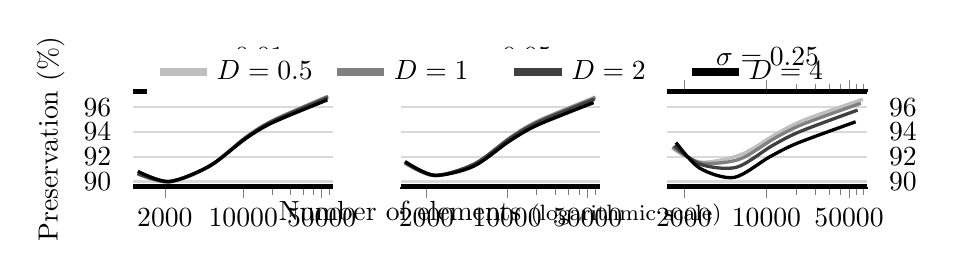
\begin{tikzpicture}
\begin{scope}[shift={(0.0\linewidth,0)}]
\begin{axis}[
 width=0.34\linewidth,height=0.23\linewidth,
 title=\normalsize\mbox{$\sigma=0.01$},
 xmode=log,enlarge x limits=0.025,
 ylabel=Preservation (\%),
 axis y line*=left,
 ymin=89.5852833333,ymax=97.2597858333,
 tick align=outside,
 x axis line style = ultra thick,y axis line style={white},
 xtick={2000,10000,50000},xticklabels={2000,10000,50000},
 minor xtick={18000,26000,34000,42000,58000,66000}, every y tick/.style={white},ymajorgrids,grid style={gray!30,thick}]
\addplot[very thick,mark=none,smooth,color=black!25] table[] {
	1142.66433333 90.6223333333
	2190.331 89.9333333333
	5024.068 91.2336666667
	10557.4073333 93.559
	18518.477 94.946
	57160.1013333 96.8943333333
};
\addplot[very thick,mark=none,smooth,color=black!50] table[] {
	1142.66433333 90.6223333333
	2203.91966667 89.983
	5019.90933333 91.2416666667
	10559.26 93.5726666667
	18496.2383333 94.9303333333
	56994.2803333 96.8676666667
};
\addplot[very thick,mark=none,smooth,color=black!75] table[] {
	1147.421 90.6463333333
	2198.01033333 89.9903333333
	5048.57 91.277
	10575.013 93.5463333333
	18463.3696667 94.888
	56796.2563333 96.7726666667
};
\addplot[very thick,mark=none,smooth,color=black] table[] {
	1148.51366667 90.8193333333
	2179.72533333 89.9976666667
	4988.35566667 91.237
	10445.26 93.4446666667
	18253.313 94.7536666667
	56234.555 96.5863333333
};
!\end{axis}
\end{scope}
\begin{scope}[shift={(0.28\linewidth,0)}]
\begin{axis}[
 width=0.34\linewidth,height=0.23\linewidth,
 title=\normalsize\mbox{$\sigma=0.05$},
 xmode=log,enlarge x limits=0.025,
 xlabel=Number of elements \footnotesize(logarithmic scale),x label style={at={(axis description cs:0.5,-0.05)},anchor=north},
 yticklabels={},
 legend style={at={(0.55,1.45)},legend style={text width=4em},legend style={draw=none},anchor=north,legend columns=-1},
 axis y line*=left,
 ymin=89.5852833333,ymax=97.2597858333,
 tick align=outside,
 x axis line style = ultra thick,y axis line style={white},
 xtick={2000,10000,50000},xticklabels={2000,10000,50000},
 minor xtick={18000,26000,34000,42000,58000,66000}, every y tick/.style={white},ymajorgrids,grid style={gray!30,thick}]
\addlegendimage{line width=3pt,mark=none,black!25}
\addlegendentry{$D=0.5$}
\addlegendimage{line width=3pt,mark=none,black!50}
\addlegendentry{$D=1$}
\addlegendimage{line width=3pt,mark=none,black!75}
\addlegendentry{$D=2$}
\addlegendimage{line width=3pt,mark=none,black}
\addlegendentry{$D=4$}
\addplot[very thick,mark=none,smooth,color=black!25] table[] {
	1298.20533333 91.495
	2340.633 90.4603333333
	5186.95033333 91.389
	10853.1023333 93.6036666667
	18943.9993333 94.9333333333
	58604.5323333 96.8286666667
};
\addplot[very thick,mark=none,smooth,color=black!50] table[] {
	1297.63266667 91.496
	2349.96633333 90.4843333333
	5211.535 91.4193333333
	10822.068 93.583
	18923.0946667 94.8986666667
	58453.4236667 96.7666666667
};
\addplot[very thick,mark=none,smooth,color=black!75] table[] {
	1302.89433333 91.533
	2349.60333333 90.4793333333
	5219.07066667 91.411
	10751.7493333 93.5096666667
	18721.5463333 94.7916666667
	57464.189 96.6476666667
};
\addplot[very thick,mark=none,smooth,color=black] table[] {
	1299.731 91.6113333333
	2327.66833333 90.506
	5087.395 91.215
	10536.52 93.2713333333
	18361.0733333 94.5533333333
	56479.5 96.3676666667
};
!\end{axis}
\end{scope}
\begin{scope}[shift={(0.56\linewidth,0)}]
\begin{axis}[
 width=0.34\linewidth,height=0.23\linewidth,
 title=\normalsize\mbox{$\sigma=0.25$},
 xmode=log,enlarge x limits=0.025,
 axis y line*=right,
 ymin=89.5852833333,ymax=97.2597858333,
 tick align=outside,
 x axis line style = ultra thick,y axis line style={white},
 xtick={2000,10000,50000},xticklabels={2000,10000,50000},
 minor xtick={18000,26000,34000,42000,58000,66000}, every y tick/.style={white},ymajorgrids,grid style={gray!30,thick}]
\addplot[very thick,mark=none,smooth,color=black!25] table[] {
	1596.30333333 92.689
	2756.53766667 91.5646666667
	6060.21733333 92.1663333333
	12338.161 93.8876666667
	21383.8163333 95.011
	65427.1206667 96.6373333333
};
\addplot[very thick,mark=none,smooth,color=black!50] table[] {
	1607.67666667 92.7946666667
	2757.58366667 91.5123333333
	5836.15333333 91.7793333333
	11813.4666667 93.507
	20455.343 94.6356666667
	63005.4993333 96.319
};
\addplot[very thick,mark=none,smooth,color=black!75] table[] {
	1656.74966667 92.8756666667
	2746.29366667 91.396
	5559.30066667 91.1436666667
	11210.0 92.8956666667
	19330.474 94.0383333333
	59102.68 95.7656666667
};
\addplot[very thick,mark=none,smooth,color=black] table[] {
	1714.92766667 93.146
	2716.32133333 91.086
	5316.24133333 90.3253333333
	10718.991 92.003
	18519.036 93.117
	56886.458 94.8183333333
};
!\end{axis}
\end{scope}
\end{tikzpicture}
\end{center}
\caption{Element preservation results using mesh remodelling}
\centering\sffamily\footnotesize
Average of thirty optimisation scenarios - RAE-2822 airfoil
\end{figure}


\paragraph{Element surplus} Another metric of some significance is element surplus, defined as the percentage of elements(triangles) in excess in meshes produced by mesh remodelling relative to the mesh generation counterparts. Its significance is derived from the fact that the more elements the mesh has, the more computations the dynamic-fluid simulators have to perform. The first remark to be made is that mesh remodelling does not achieve good results for coarse meshes, reaching values up to 50\% for larger magnitudes of model perturbations. Also note that the method achieves negative values of element surplus when performing smaller perturbations to the airfoil in very small meshes, a result derived from bad gradation. For medium-to-large meshes though, mesh remodelling achieves very good results, usually below 10\%. The increase in removal distance also has a positive impact on the results, which is more noticeable on finer meshes, with a reduction of element surplus to below 5\%, despite the also decrease in element preservation by 2\%.

\begin{figure}[!h]
\begin{center}
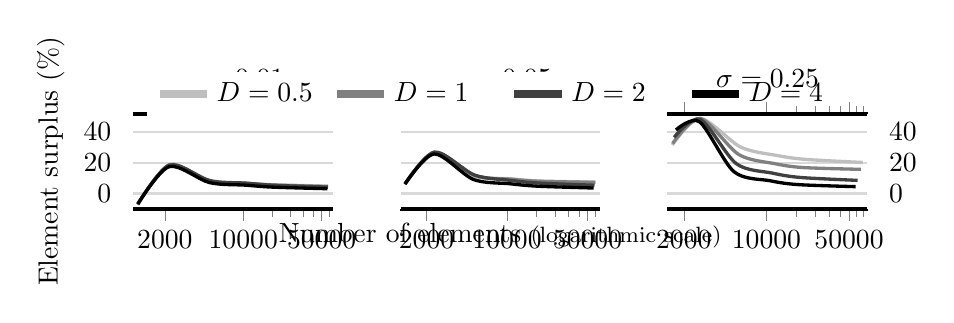
\begin{tikzpicture}
\begin{scope}[shift={(0.0\linewidth,0)}]
\begin{axis}[
 width=0.34\linewidth,height=0.23\linewidth,
 title=\normalsize\mbox{$\sigma=0.01$},
 xmode=log,enlarge x limits=0.025,
 ylabel=Element surplus (\%),
 axis y line*=left,
 ymin=-9.99254435348,ymax=51.7132290624,
 tick align=outside,
 x axis line style = ultra thick,y axis line style={white},
 xtick={2000,10000,50000},xticklabels={2000,10000,50000},
 minor xtick={18000,26000,34000,42000,58000,66000}, every y tick/.style={white},ymajorgrids,grid style={gray!30,thick}]
\addplot[very thick,mark=none,smooth,color=black!25] table[] {
	1142.66433333 -7.19409657952
	2190.331 18.0292948627
	5024.068 7.89971733263
	10557.4073333 6.5949868196
	18518.477 5.68929699423
	57160.1013333 4.84824826573
};
\addplot[very thick,mark=none,smooth,color=black!50] table[] {
	1142.66433333 -7.19409657952
	2203.91966667 18.7615406944
	5019.90933333 7.81040346231
	10559.26 6.61369264127
	18496.2383333 5.56237570118
	56994.2803333 4.54408433022
};
\addplot[very thick,mark=none,smooth,color=black!75] table[] {
	1147.421 -6.80776549839
	2198.01033333 18.4431073405
	5048.57 8.42593610078
	10575.013 6.77274597457
	18463.3696667 5.37478650186
	56796.2563333 4.18085072793
};
\addplot[very thick,mark=none,smooth,color=black] table[] {
	1148.51366667 -6.71902034885
	2179.72533333 17.4577924924
	4988.35566667 7.13273912454
	10445.26 5.46266870957
	18253.313 4.17594377689
	56234.555 3.15052713727
};
!\end{axis}
\end{scope}
\begin{scope}[shift={(0.28\linewidth,0)}]
\begin{axis}[
 width=0.34\linewidth,height=0.23\linewidth,
 title=\normalsize\mbox{$\sigma=0.05$},
 xmode=log,enlarge x limits=0.025,
 xlabel=Number of elements \footnotesize(logarithmic scale),x label style={at={(axis description cs:0.5,-0.05)},anchor=north},
 yticklabels={},
 legend style={at={(0.55,1.45)},legend style={text width=4em},legend style={draw=none},anchor=north,legend columns=-1},
 axis y line*=left,
 ymin=-9.99254435348,ymax=51.7132290624,
 tick align=outside,
 x axis line style = ultra thick,y axis line style={white},
 xtick={2000,10000,50000},xticklabels={2000,10000,50000},
 minor xtick={18000,26000,34000,42000,58000,66000}, every y tick/.style={white},ymajorgrids,grid style={gray!30,thick}]
\addlegendimage{line width=3pt,mark=none,black!25}
\addlegendentry{$D=0.5$}
\addlegendimage{line width=3pt,mark=none,black!50}
\addlegendentry{$D=1$}
\addlegendimage{line width=3pt,mark=none,black!75}
\addlegendentry{$D=2$}
\addlegendimage{line width=3pt,mark=none,black}
\addlegendentry{$D=4$}
\addplot[very thick,mark=none,smooth,color=black!25] table[] {
	1298.20533333 6.06322045678
	2340.633 26.4079832236
	5186.95033333 11.3377964278
	10853.1023333 9.57867583198
	18943.9993333 8.11295780414
	58604.5323333 7.50044176941
};
\addplot[very thick,mark=none,smooth,color=black!50] table[] {
	1297.63266667 6.01643365861
	2349.96633333 26.9120382563
	5211.535 11.8655058595
	10822.068 9.26533674722
	18923.0946667 7.99365536406
	58453.4236667 7.22325760336
};
\addplot[very thick,mark=none,smooth,color=black!75] table[] {
	1302.89433333 6.44631119593
	2349.60333333 26.892434116
	5219.07066667 12.0272588102
	10751.7493333 8.55536220326
	18721.5463333 6.84342377496
	57464.189 5.40866819455
};
\addplot[very thick,mark=none,smooth,color=black] table[] {
	1299.731 6.18786724096
	2327.66833333 25.7078147792
	5087.395 9.20084297278
	10536.52 6.3822927322
	18361.0733333 4.78621285805
	56479.5 3.60241706872
};
!\end{axis}
\end{scope}
\begin{scope}[shift={(0.56\linewidth,0)}]
\begin{axis}[
 width=0.34\linewidth,height=0.23\linewidth,
 title=\normalsize\mbox{$\sigma=0.25$},
 xmode=log,enlarge x limits=0.025,
 axis y line*=right,
 ymin=-9.99254435348,ymax=51.7132290624,
 tick align=outside,
 x axis line style = ultra thick,y axis line style={white},
 xtick={2000,10000,50000},xticklabels={2000,10000,50000},
 minor xtick={18000,26000,34000,42000,58000,66000}, every y tick/.style={white},ymajorgrids,grid style={gray!30,thick}]
\addplot[very thick,mark=none,smooth,color=black!25] table[] {
	1596.30333333 31.5342999505
	2756.53766667 48.7184259783
	6060.21733333 30.1597822272
	12338.161 24.6954469507
	21383.8163333 22.1880437805
	65427.1206667 20.1757517151
};
\addplot[very thick,mark=none,smooth,color=black!50] table[] {
	1607.67666667 32.4714548176
	2757.58366667 48.7748588997
	5836.15333333 25.3473935221
	11813.4666667 19.3926312064
	20455.343 16.8827073272
	63005.4993333 15.7277466503
};
\addplot[very thick,mark=none,smooth,color=black!75] table[] {
	1656.74966667 36.5150363642
	2746.29366667 48.1657502162
	5559.30066667 19.4012234724
	11210.0 13.2937040064
	19330.474 10.4551576103
	59102.68 8.55909483723
};
\addplot[very thick,mark=none,smooth,color=black] table[] {
	1714.92766667 41.3088636668
	2716.32133333 46.5487078336
	5316.24133333 14.1808579055
	10718.991 8.33132859961
	18519.036 5.81856607198
	56886.458 4.48836480809
};
!\end{axis}
\end{scope}
\end{tikzpicture}
\end{center}
\caption{Element surplus results on meshes from mesh remodelling when compared to those from mesh generation}
\centering\sffamily\footnotesize
Average of thirty optimisation scenarios - RAE-2822 airfoil
\end{figure}


\paragraph{Speed-up} Perhaps the most impressive results, although the less important, are related to the time of execution. The speed-ups achieved by using mesh remodelling instead of mesh generation can vary greatly, from fifteen in larger perturbations to sixty in slighter ones. Even so, the results are as expected; the speed-up rises as mesh resolution increases and falls as either removal distance or the magnitude of the model perturbations increases.

\begin{figure}[!h]
\begin{center}
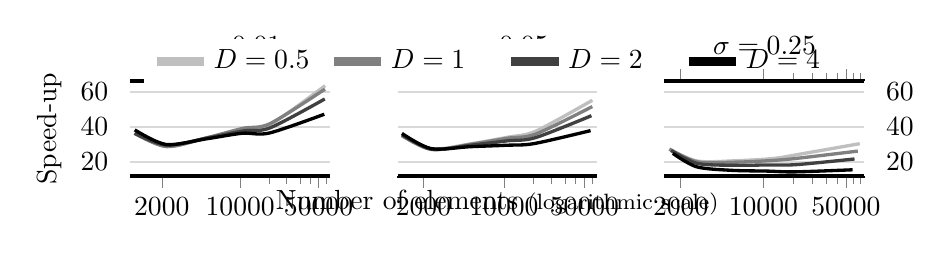
\begin{tikzpicture}
\begin{scope}[shift={(0.0\linewidth,0)}]
\begin{axis}[
 width=0.34\linewidth,height=0.23\linewidth,
 title=\normalsize\mbox{$\sigma=0.01$},
 xmode=log,enlarge x limits=0.025,
 ylabel=Speed-up,
 axis y line*=left,
 ymin=11.6727451262,ymax=66.0907077262,
 tick align=outside,
 x axis line style = ultra thick,y axis line style={white},
 xtick={2000,10000,50000},xticklabels={2000,10000,50000},
 minor xtick={18000,26000,34000,42000,58000,66000}, every y tick/.style={white},ymajorgrids,grid style={gray!30,thick}]
\addplot[very thick,mark=none,smooth,color=black!25] table[] {
	1142.66433333 36.2897800776
	2190.331 28.7700165654
	5024.068 33.6092943201
	10557.4073333 38.7642733564
	18518.477 41.2486285483
	57160.1013333 63.4993761738
};
\addplot[very thick,mark=none,smooth,color=black!50] table[] {
	1142.66433333 36.2897800776
	2203.91966667 28.5963227223
	5019.90933333 33.6092943201
	10559.26 39.0416951895
	18496.2383333 41.7761950928
	56994.2803333 61.4995484552
};
\addplot[very thick,mark=none,smooth,color=black!75] table[] {
	1147.421 36.1727917473
	2198.01033333 29.3866328257
	5048.57 33.4748571429
	10575.013 37.5305695142
	18463.3696667 39.3203242902
	56796.2563333 55.8640439053
};
\addplot[very thick,mark=none,smooth,color=black] table[] {
	1148.51366667 38.1659863946
	2179.72533333 29.8325221872
	4988.35566667 33.0443366426
	10445.26 36.2385050832
	18253.313 36.3940358628
	56234.555 47.1214037892
};
!\end{axis}
\end{scope}
\begin{scope}[shift={(0.28\linewidth,0)}]
\begin{axis}[
 width=0.34\linewidth,height=0.23\linewidth,
 title=\normalsize\mbox{$\sigma=0.05$},
 xmode=log,enlarge x limits=0.025,
 xlabel=Number of elements \footnotesize(logarithmic scale),x label style={at={(axis description cs:0.5,-0.05)},anchor=north},
 yticklabels={},
 legend style={at={(0.55,1.45)},legend style={text width=4em},legend style={draw=none},anchor=north,legend columns=-1},
 axis y line*=left,
 ymin=11.6727451262,ymax=66.0907077262,
 tick align=outside,
 x axis line style = ultra thick,y axis line style={white},
 xtick={2000,10000,50000},xticklabels={2000,10000,50000},
 minor xtick={18000,26000,34000,42000,58000,66000}, every y tick/.style={white},ymajorgrids,grid style={gray!30,thick}]
\addlegendimage{line width=3pt,mark=none,black!25}
\addlegendentry{$D=0.5$}
\addlegendimage{line width=3pt,mark=none,black!50}
\addlegendentry{$D=1$}
\addlegendimage{line width=3pt,mark=none,black!75}
\addlegendentry{$D=2$}
\addlegendimage{line width=3pt,mark=none,black}
\addlegendentry{$D=4$}
\addplot[very thick,mark=none,smooth,color=black!25] table[] {
	1298.20533333 34.9249530957
	2340.633 27.2511798637
	5186.95033333 30.2464011768
	10853.1023333 34.0036383991
	18943.9993333 37.479457559
	58604.5323333 55.1570578358
};
\addplot[very thick,mark=none,smooth,color=black!50] table[] {
	1297.63266667 34.903125
	2349.96633333 26.9194509195
	5211.535 29.9973947478
	10822.068 33.4383772775
	18923.0946667 35.8195142245
	58453.4236667 51.5111855511
};
\addplot[very thick,mark=none,smooth,color=black!75] table[] {
	1302.89433333 35.4346446701
	2349.60333333 27.1302531976
	5219.07066667 29.4661684922
	10751.7493333 31.9152569087
	18721.5463333 33.7135628445
	57464.189 46.2930500561
};
\addplot[very thick,mark=none,smooth,color=black] table[] {
	1299.731 36.145631068
	2327.66833333 27.4599735799
	5087.395 28.5513786947
	10536.52 29.375
	18361.0733333 30.3578422066
	56479.5 37.7507056018
};
!\end{axis}
\end{scope}
\begin{scope}[shift={(0.56\linewidth,0)}]
\begin{axis}[
 width=0.34\linewidth,height=0.23\linewidth,
 title=\normalsize\mbox{$\sigma=0.25$},
 xmode=log,enlarge x limits=0.025,
 axis y line*=right,
 ymin=11.6727451262,ymax=66.0907077262,
 tick align=outside,
 x axis line style = ultra thick,y axis line style={white},
 xtick={2000,10000,50000},xticklabels={2000,10000,50000},
 minor xtick={18000,26000,34000,42000,58000,66000}, every y tick/.style={white},ymajorgrids,grid style={gray!30,thick}]
\addplot[very thick,mark=none,smooth,color=black!25] table[] {
	1596.30333333 27.2734915925
	2756.53766667 20.3341269841
	6060.21733333 20.5562134613
	12338.161 21.8514300457
	21383.8163333 24.5252219532
	65427.1206667 30.2779874294
};
\addplot[very thick,mark=none,smooth,color=black!50] table[] {
	1607.67666667 27.1392716535
	2757.58366667 19.8998058252
	5836.15333333 19.7054892944
	11813.4666667 20.6324343136
	20455.343 22.0838397093
	63005.4993333 26.0327366598
};
\addplot[very thick,mark=none,smooth,color=black!75] table[] {
	1656.74966667 26.3861244019
	2746.29366667 19.0243178021
	5559.30066667 17.9208703607
	11210.0 18.1140543844
	19330.474 18.3126255524
	59102.68 21.5156095705
};
\addplot[very thick,mark=none,smooth,color=black] table[] {
	1714.92766667 24.7185118781
	2716.32133333 17.0579227696
	5316.24133333 15.0370634355
	10718.991 14.5844628668
	18519.036 14.140679938
	56886.458 15.3270226751
};
!\end{axis}
\end{scope}
\end{tikzpicture}
\end{center}
\caption{Speed-up results by mesh remodelling relative to mesh generation}
\centering\sffamily\footnotesize
Average of thirty optimisation scenarios - RAE-2822 airfoil
\end{figure}


\begin{figure}[!h]
\begin{center}
%	\input{figures/mesh_d1}
%	\input{figures/mesh_d4}
\begin{subfigure}{0.49\linewidth}
	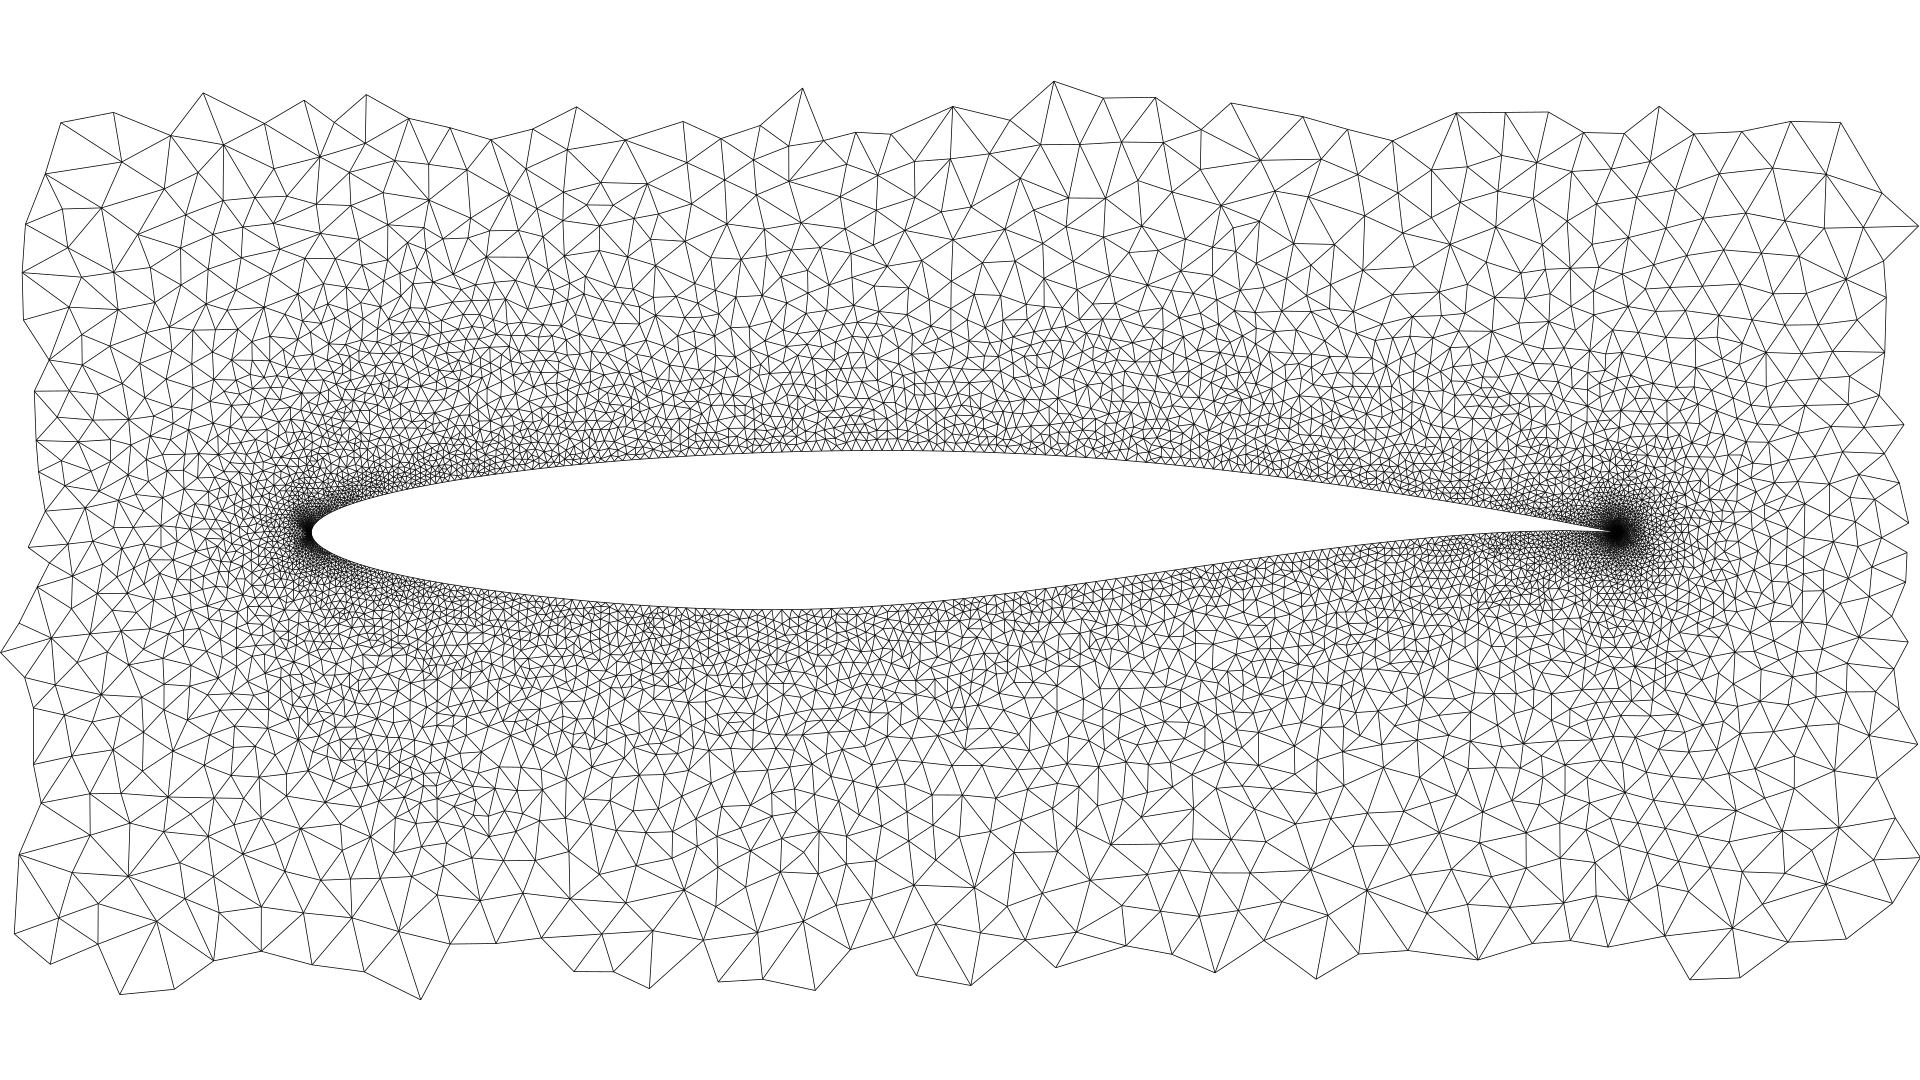
\includegraphics[width=\linewidth]{pictures/mesh_d1}
	\caption{$D=1$}
\end{subfigure}
\hspace{0.01\linewidth}
\begin{subfigure}{0.49\linewidth}
	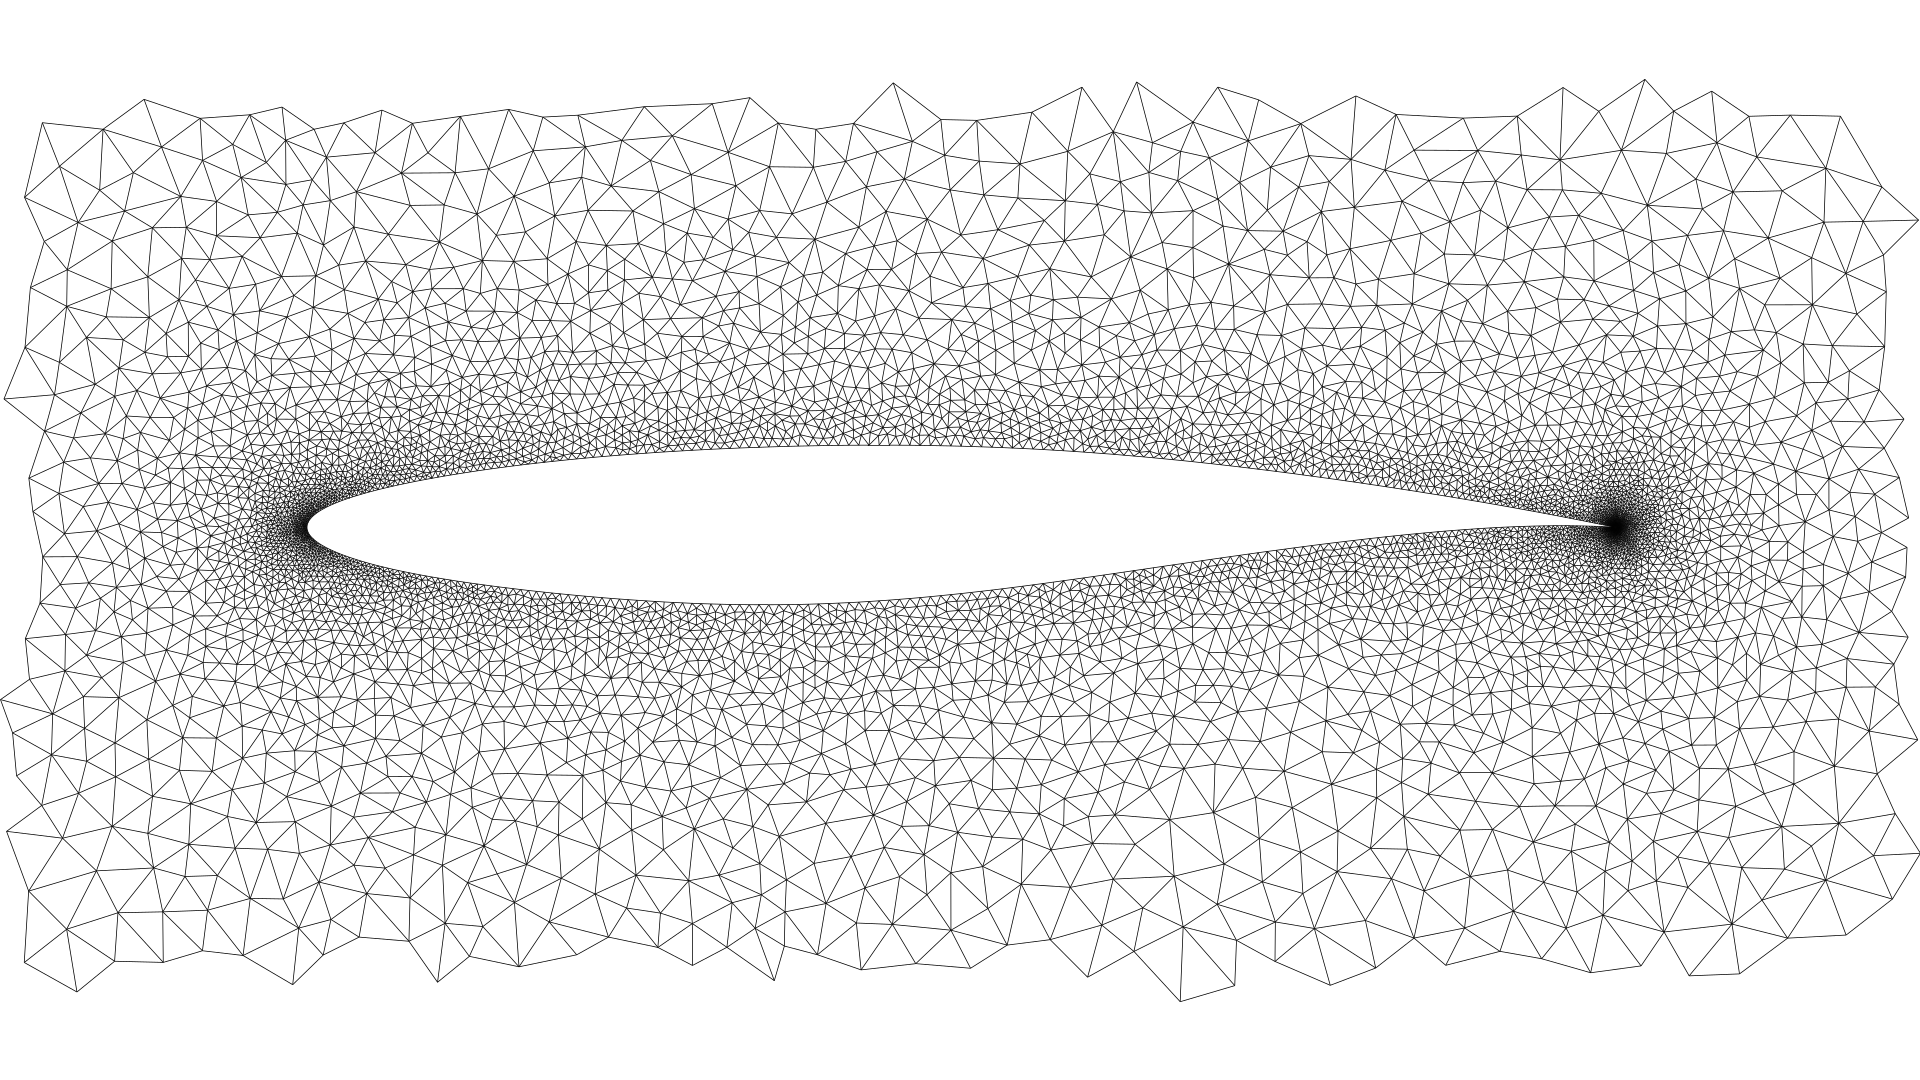
\includegraphics[width=\linewidth]{pictures/mesh_d4}
	\caption{$D=4$}
\end{subfigure}
\end{center}
\caption{Illustration of element surplus and bad gradation\\\footnotesize Mesh remodelling, $\sigma=0.25, I=400, G=8$, RAE-2822 airfoil}
\end{figure}

\paragraph{Improvements} Despite the good results, there is still room for improvement, especially concerning the problem of element surplus and bad gradation. One possible strategy, that follows from a previous work where its development and testing was carried out, involves choosing which method to perform --- generation or remodelling --- at a given iteration. The criteria for such decision can include the variation in the shape coefficient vector, $A$, the current value of element surplus --- although difficult to control, given that there is no point of comparison and that the higher number of elements could just be a consequence of a thinner model --- or even be a periodic event. One other alternative is as follows. In this work's particular case, due to the way the CMA-ES works, it is almost certain that at some point during the nine thousand iterations --- depending on the value of $\sigma$ --- the mesh remodelling method will start performing only full adjustments (adjust  all vertices) until the very end. One can take advantage of such behaviour and upon detecting, for example, ten successive full adjustments, instruct the program to perform a single mesh generation iteration. Since the remaining iterations are bound to be full adjustments, it is guaranteed that no elements will be either added or removed from the mesh, which results in an element surplus of 0\% from that point onwards at the cost of a merely one-hundredth of a percent in element preservation in the end. Ultimately, all possible improvements are to be considered from the fluid-dynamics simulator's point of view.